\subsection{Results}

\subsubsection{H1: a fixed gate yields higher worst-group accuracy than a learned gate}

\textbf{Target and test.}

\begin{itemize}
\tightlist
\item
  Target: H1, fixed gate \textgreater{} learned gate.
\item
  Test: one-sided paired t-test over seeds, with the Wilcoxon signed-rank test as an assumption-free check
  (Table 1, Figure 1).
\end{itemize}

\textbf{Verdict: supported for Qwen3.5-4B on both tasks.}

\begin{itemize}
\tightlist
\item
  \emph{Waterbirds:} the fixed gate exceeds the learned gate by 10.6 points.

  \begin{itemize}
  \tightlist
  \item
    Paired test: 95\% CI {[}5.3, 16.0{]}, t(14) = 4.26, p = 4.0 × 10⁻⁴, \(d_z\) = 1.10.
  \item
    Wilcoxon: p = 3.1 × 10⁻⁵.
  \end{itemize}
\item
  \emph{Watermark:} the gain is 25.2 points.

  \begin{itemize}
  \tightlist
  \item
    Paired test: 95\% CI {[}14.8, 35.6{]}, t(14) = 5.21, p = 6.6 × 10⁻⁵, \(d_z\) = 1.34.
  \item
    Wilcoxon: p = 6.1 × 10⁻⁵.
  \end{itemize}
\item
  Both effects are large by conventional thresholds \cite{cohen1988power}. Achieved power is 0.98 and 0.99.
\item
  \emph{Robustness of the verdict} (\texttt{results\_study/robustness\_checks.md}):

  \begin{itemize}
  \item
    Unpaired tests, which do not rely on seed pairing, agree: Welch p = 7.6 × 10⁻⁴ and 5.1 × 10⁻⁵;
    Mann--Whitney p = 1.2 × 10⁻⁵ and 2.5 × 10⁻⁴.
  \item
    With label-free model selection (best validation average accuracy) the gain is +17.7 and +25.5
    (paired p = 0.002 and 6.0 × 10⁻⁵), so it does not depend on using group labels for selection.
  \item
    The fixed gate also raises average accuracy (84.1 → 88.0, p = 0.007; 76.9 → 86.1, p = 7.4 × 10⁻⁴), with
    in-distribution accuracy unchanged (≈ 98\%). The worst-group gain is not a trade-off against accuracy.
  \item
    \emph{Confirmation sample.} H1 was formed after a 3-seed pilot, so it is also tested on the later seeds only:
    Waterbirds +10.5 (12 seeds, t(11) = 4.06, p = 9.5 × 10⁻⁴, \(d_z\) = 1.17); Watermark +26.7 (12 seeds,
    t(11) = 4.86, p = 2.5 × 10⁻⁴, \(d_z\) = 1.40). The pilot alone was not significant (p = 0.16 and 0.12).
  \item
    \emph{Multiplicity.} With Holm correction across the four H1 tests (2 LLMs × 2 tasks), all four survive at 0.025
    (adjusted p = 0.0012 and 2.7 × 10⁻⁴ for Qwen3.5-4B, 0.0086 and 0.0086 for Phi-4-mini;
    \texttt{results\_study/extra\_analyses.md} §1).
  \end{itemize}
\end{itemize}

\textbf{Phi-4-mini, second LLM.}

\begin{itemize}
\item
  \emph{Waterbirds:} H1 is supported (+9.7, t(4) = 4.52, p = 0.005, \(d_z\) = 2.02).
\item
  \emph{Watermark, 10 seeds:} H1 is supported (+25.5, 95\% CI {[}8.2, 42.7{]}, t(9) = 3.34, p = 0.0043,
  Wilcoxon p = 9.8 × 10⁻⁴, \(d_z\) = 1.06).

  \begin{itemize}
  \item
    With the first 5 seeds the gain (+31.6) missed α = 0.025 (p = 0.044). Seeds 5--9 were added \emph{after} that
    result, to reach the ≈ 10 seeds a power analysis asked for. Because the extension depended on the first
    result, it is also tested on the new seeds alone, which are fresh data: +19.4, t(4) = 2.88, p = 0.023,
    fixed \textgreater{} learned in 5 of 5.
  \item
    The fixed gate is not robust on this task either: 6 of 10 fixed-gate seeds fall below 50\% WGA (8 of 10
    learned). Phi-4-mini finds the watermark task harder with any gate.
  \end{itemize}
\end{itemize}

\textbf{Table 1.} Gate hypotheses (WGA, \%).

{\def\LTcaptype{none} % do not increment counter
\begin{longtable}[]{@{}
  >{\raggedright\arraybackslash}p{(\linewidth - 20\tabcolsep) * \real{0.0755}}
  >{\raggedright\arraybackslash}p{(\linewidth - 20\tabcolsep) * \real{0.0755}}
  >{\centering\arraybackslash}p{(\linewidth - 20\tabcolsep) * \real{0.0943}}
  >{\centering\arraybackslash}p{(\linewidth - 20\tabcolsep) * \real{0.0943}}
  >{\centering\arraybackslash}p{(\linewidth - 20\tabcolsep) * \real{0.0943}}
  >{\centering\arraybackslash}p{(\linewidth - 20\tabcolsep) * \real{0.0943}}
  >{\centering\arraybackslash}p{(\linewidth - 20\tabcolsep) * \real{0.0943}}
  >{\centering\arraybackslash}p{(\linewidth - 20\tabcolsep) * \real{0.0943}}
  >{\centering\arraybackslash}p{(\linewidth - 20\tabcolsep) * \real{0.0943}}
  >{\centering\arraybackslash}p{(\linewidth - 20\tabcolsep) * \real{0.0943}}
  >{\centering\arraybackslash}p{(\linewidth - 20\tabcolsep) * \real{0.0943}}@{}}
\toprule\noalign{}
\begin{minipage}[b]{\linewidth}\raggedright
LLM
\end{minipage} & \begin{minipage}[b]{\linewidth}\raggedright
Task
\end{minipage} & \begin{minipage}[b]{\linewidth}\centering
Seeds
\end{minipage} & \begin{minipage}[b]{\linewidth}\centering
Learned
\end{minipage} & \begin{minipage}[b]{\linewidth}\centering
Fixed
\end{minipage} & \begin{minipage}[b]{\linewidth}\centering
Δ {[}95\% CI{]}
\end{minipage} & \begin{minipage}[b]{\linewidth}\centering
t (df)
\end{minipage} & \begin{minipage}[b]{\linewidth}\centering
p (t)
\end{minipage} & \begin{minipage}[b]{\linewidth}\centering
p (Wilcoxon)
\end{minipage} & \begin{minipage}[b]{\linewidth}\centering
\(d_z\)
\end{minipage} & \begin{minipage}[b]{\linewidth}\centering
Collapsed \textless{} 50 (L / F)
\end{minipage} \\
\midrule\noalign{}
\endhead
\bottomrule\noalign{}
\endlastfoot
Qwen3.5-4B & Waterbirds & 15 & 63.6 ± 10.4 & 74.2 ± 3.4 & +10.6 {[}5.3, 16.0{]} & 4.26 (14) & 4.0e-4 & 3.1e-5 & 1.10 & 2 / 0 \\
Qwen3.5-4B & Watermark & 15 & 40.5 ± 18.0 & 65.7 ± 10.3 & +25.2 {[}14.8, 35.6{]} & 5.21 (14) & 6.6e-5 & 6.1e-5 & 1.34 & 10 / 0 \\
Phi-4-mini & Waterbirds & 5 & 60.4 ± 5.7 & 70.1 ± 3.6 & +9.7 {[}3.8, 15.7{]} & 4.52 (4) & 5.3e-3 & 3.1e-2 & 2.02 & 0 / 0 \\
Phi-4-mini & Watermark & 10 & 29.4 ± 18.7 & 54.9 ± 14.5 & +25.5 {[}8.2, 42.7{]} & 3.34 (9) & 4.3e-3 & 9.8e-4 & 1.06 & 8 / 6 \\
\end{longtable}
}

With n = 5 the smallest attainable one-sided Wilcoxon p is 0.031, so the Wilcoxon test cannot reach
α = 0.025 for Phi-4-mini Waterbirds. Figure 1: \texttt{results\_study/h1\_gate\_seeds.png}, \texttt{results\_study/phi/h1\_gate\_seeds.png}
(one line per seed).

Figure \ref{fig:main} shows every seed of the four connectors, and Figure \ref{fig:forest} the paired gain with its 95\% interval in all four LLM × task cells.

\begin{figure}[t]
\centering
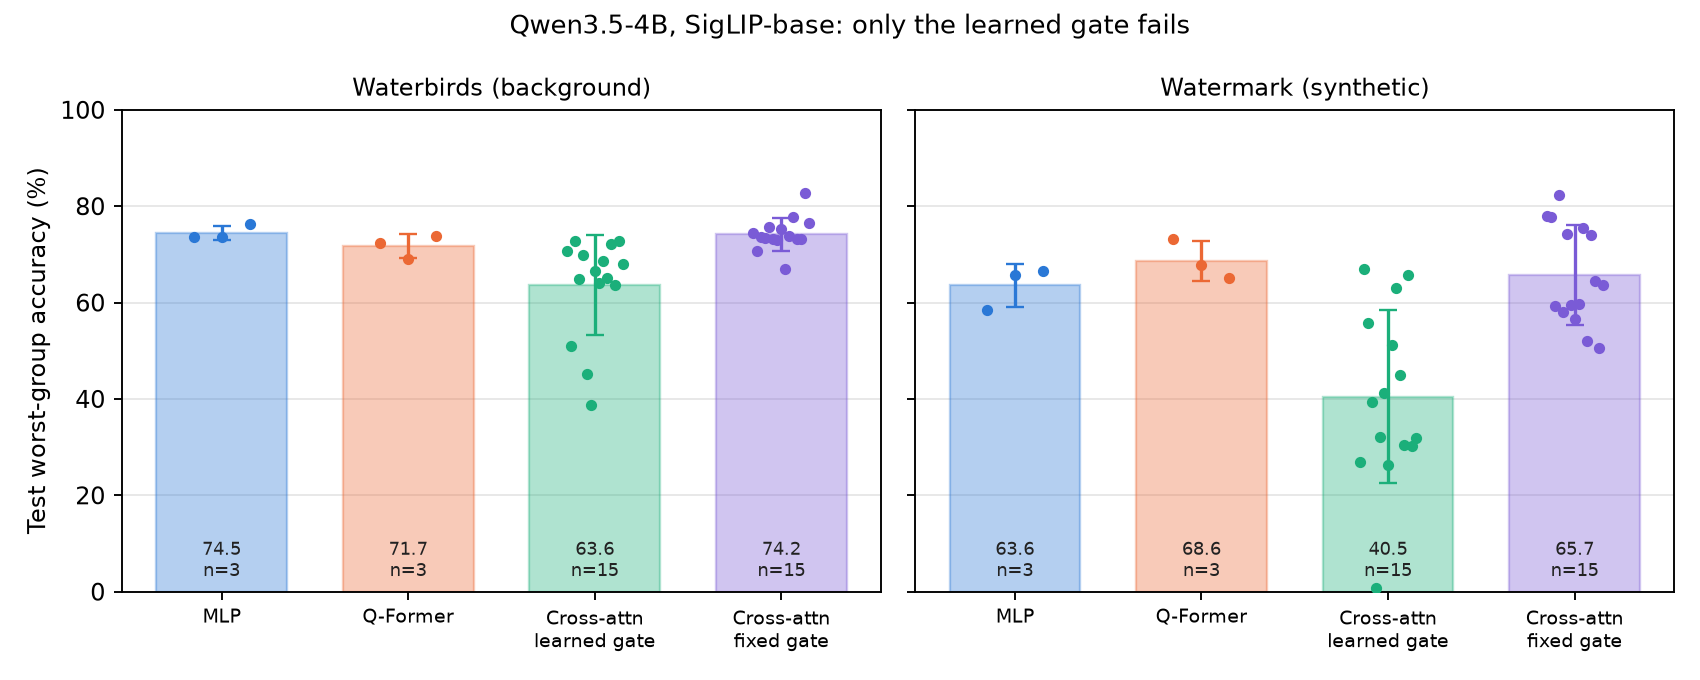
\includegraphics[width=\linewidth]{figures/main_connectors.png}
\caption{Test worst-group accuracy of the four connectors (Qwen3.5-4B, SigLIP-base). Bars are means over seeds; dots are individual seeds. Only the learnable, zero-initialised gate fails, and it is also the least stable.}\label{fig:main}
\end{figure}

\textbackslash begin\{figure\}{[}t{]}
\centering
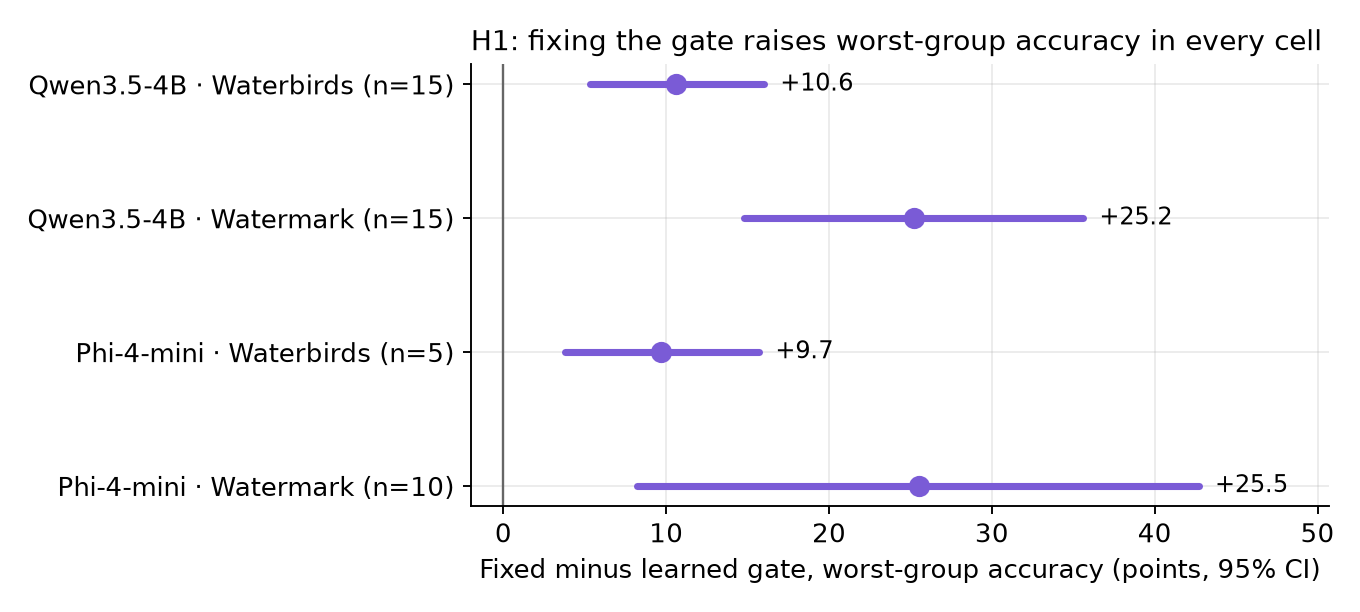
\includegraphics[width=0.85\linewidth]{figures/forest_gain.png}
\textbackslash caption\{Paired gain from fixing the gate (fixed minus learnable gate, worst-group accuracy points) with 95\% confidence intervals, for both LLMs and both tasks. All four cells survive Holm correction.\}\label{fig:forest}
\textbackslash end\{figure\}

\subsubsection{H2: the learned gate is less stable across seeds}

\textbf{Target and test.}

\begin{itemize}
\tightlist
\item
  Target: H2, the learned gate is more variable.
\item
  Test: one-sided F-test on seed variances, with the Brown--Forsythe test as a robust check, since learned-gate
  WGA is non-normal on Qwen Waterbirds (Shapiro--Wilk p = 0.003).
\end{itemize}

\textbf{Verdict: supported for Qwen3.5-4B, by different tests on the two tasks.} The variance tests and a count of
collapsed runs (Fisher's exact test, which assumes nothing about the distribution) are reported side by side
(\texttt{results\_study/extra\_analyses.md} §1b).

{\def\LTcaptype{none} % do not increment counter
\begin{longtable}[]{@{}
  >{\raggedright\arraybackslash}p{(\linewidth - 10\tabcolsep) * \real{0.1600}}
  >{\raggedright\arraybackslash}p{(\linewidth - 10\tabcolsep) * \real{0.1600}}
  >{\raggedright\arraybackslash}p{(\linewidth - 10\tabcolsep) * \real{0.1600}}
  >{\centering\arraybackslash}p{(\linewidth - 10\tabcolsep) * \real{0.2000}}
  >{\raggedright\arraybackslash}p{(\linewidth - 10\tabcolsep) * \real{0.1600}}
  >{\raggedright\arraybackslash}p{(\linewidth - 10\tabcolsep) * \real{0.1600}}@{}}
\toprule\noalign{}
\begin{minipage}[b]{\linewidth}\raggedright
Task
\end{minipage} & \begin{minipage}[b]{\linewidth}\raggedright
F-test (one-sided)
\end{minipage} & \begin{minipage}[b]{\linewidth}\raggedright
Brown--Forsythe (two-sided)
\end{minipage} & \begin{minipage}[b]{\linewidth}\centering
Collapsed \textless{} 50, learned / fixed
\end{minipage} & \begin{minipage}[b]{\linewidth}\raggedright
Fisher exact (one-sided)
\end{minipage} & \begin{minipage}[b]{\linewidth}\raggedright
Reading
\end{minipage} \\
\midrule\noalign{}
\endhead
\bottomrule\noalign{}
\endlastfoot
Waterbirds & F = 9.2, p = 8.6 × 10⁻⁵ & p = 0.045 & 2 / 15 vs 0 / 15 & p = 0.24 & More variable; collapses rare \\
Watermark & F = 3.1, p = 0.023 & p = 0.097 & 10 / 15 vs 0 / 15 & p = 1.0 × 10⁻⁴ & Collapses far more often \\
\end{longtable}
}

\begin{itemize}
\item
  On Waterbirds the learned gate spreads more but rarely collapses; on Watermark the spread test is weak but
  collapses are frequent with the learned gate and absent with the fixed gate. The ``seed lottery'' claim rests
  on the collapse count, which is the quantity a practitioner cares about.
\item
  Learned-gate WGA is non-normal on Waterbirds (Shapiro--Wilk p = 0.003), so the F-test there is backed by
  Brown--Forsythe.
\item
  For Phi-4-mini no instability test is significant (F p = 0.20 and 0.23; collapses 0/0 and 8/6). H2 is not
  claimed for Phi-4-mini.
\end{itemize}

Figure \ref{fig:seeds} pairs each seed's learnable-gate and fixed-gate runs.

\begin{figure}[t]
\centering
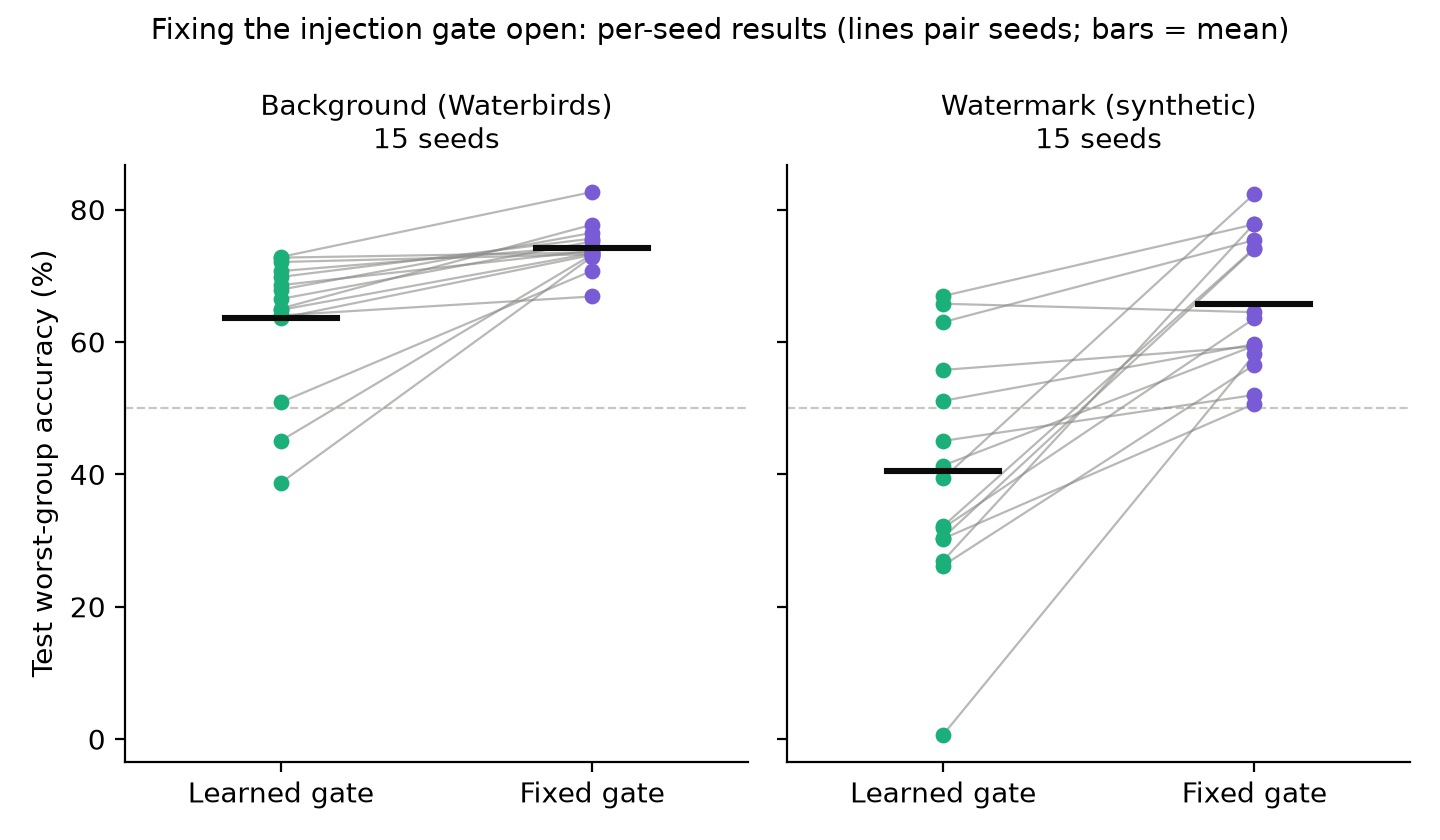
\includegraphics[width=0.85\linewidth]{figures/h1_seeds_qwen.png}
\caption{Each line joins one seed's learnable-gate run to its fixed-gate run (Qwen3.5-4B). The learnable gate collapses on many seeds; the fixed gate on none.}\label{fig:seeds}
\end{figure}

\subsubsection{Mechanism: the learned gate stays closed}

\textbf{Target.} Exploratory: whether the gate opens. It is initialised at 0 (tanh 0 = 0), so the question is
whether training opens it, not whether it closes.

\textbf{Gate value.}

\begin{itemize}
\item
  After 300 alignment steps, \textbar tanh α\textbar{} = 0.0005 with SigLIP-base and 0.0006 with SigLIP-large.
\item
  It never opens: in the logged trace it peaks at about 0.006 within 20 steps and decays to ≈ 0.001.
\item
  The logged gradient is near ±1 and changes sign between logged steps (\texttt{align.json}, \texttt{gate\_trace}). It is the
  value \emph{after} global-norm clipping at 1, so it means the gate's gradient made up almost all of the clipped
  norm, not that its raw gradient is 1. Global clipping therefore shrinks every other connector update when the
  gate is learnable. Flamingo uses the same clipping; a control that leaves the gate out of clipping, and raw
  gradient logging, are in round 5.
\item
  A small gate is not by itself a small injection, because \texttt{out\_proj} is unconstrained and can grow to
  offset it. The injected signal \texttt{‖tanh(α)·out\_proj(attn)‖\ /\ ‖e‖} is therefore logged on every evaluation
  from round 4 on (\texttt{inject\_ratio}), for SigLIP-base and SigLIP-large.
\item
  \emph{Result (\texttt{results\_study/extra\_analyses.md} §6):} \texttt{out\_proj} does partly compensate. With tanh α ≈ 0.003 the
  learned gate still injects 1.2--7.5 times the text-embedding norm (mean 3.5, Qwen, 6 runs), but the fixed
  gate injects 95--129 (mean 112) and the open gate 106--145. The learned gate passes 15--35× less visual
  signal. Within learned-gate runs the ratio does not predict WGA (Spearman ρ = 0.33, p = 0.27, 13 runs).
\item
  \emph{Longer alignment does not open the gate (§4):} after 3,000 alignment steps instead of 300 the gate peaks at
  \textbar tanh α\textbar{} = 0.003 and ends at −0.0002. The learned-gate alignment also diverged: its captioning loss fell to
  2.0 by step \textasciitilde310, then rose to 7.9, while the fixed gate's ended at 2.5. With the gate near zero, a large loss can only come
  from \texttt{out\_proj} growing until the small gated term disrupts the embeddings, so the product parametrisation
  \texttt{tanh(α)·out\_proj} is itself unstable over long training.
\end{itemize}

\textbf{Attention on the shortcut.} Both cross-attention variants attend to the watermark corner more when it is
present (uniform share 8.2\%):

{\def\LTcaptype{none} % do not increment counter
\begin{longtable}[]{@{}lcc@{}}
\toprule\noalign{}
Variant & Watermark present & Watermark absent \\
\midrule\noalign{}
\endhead
\bottomrule\noalign{}
\endlastfoot
Learned gate & 16.7\% & 6.1\% \\
Fixed gate & 18.2\% & 7.0\% \\
\end{longtable}
}

Yet only the learned gate fails.

\textbf{Released checkpoints.} Gates with \textbar tanh α\textbar{} \textless{} 0.05:

\begin{itemize}
\item
  IDEFICS-80B: 9 of 20 cross-attention layers. IDEFICS-9B: 1 of 8.
\item
  Llama 3.2 Vision: all of them. Mean \textbar tanh α\textbar{} is 0.003 at 11B (8 of 8 layers) and 0.001 at 90B (20 of 20).
  Values rise with depth (0.001 at layer 3 to 0.009 at layer 38 in 11B).
\item
  These fully trained models clearly use the image, so a small gate there must be offset by large
  cross-attention outputs. The gate parameter alone is therefore not a measure of transmitted signal, which is
  why we add the injection ratio and the ablation test.
\end{itemize}

\subsubsection{Connector type, once the gate is fixed}

\textbf{Test.} Paired t-test over 5 seeds, plus TOST with a ±3-point margin.

{\def\LTcaptype{none} % do not increment counter
\begin{longtable}[]{@{}
  >{\raggedright\arraybackslash}p{(\linewidth - 8\tabcolsep) * \real{0.1739}}
  >{\centering\arraybackslash}p{(\linewidth - 8\tabcolsep) * \real{0.2174}}
  >{\centering\arraybackslash}p{(\linewidth - 8\tabcolsep) * \real{0.2174}}
  >{\centering\arraybackslash}p{(\linewidth - 8\tabcolsep) * \real{0.2174}}
  >{\raggedright\arraybackslash}p{(\linewidth - 8\tabcolsep) * \real{0.1739}}@{}}
\toprule\noalign{}
\begin{minipage}[b]{\linewidth}\raggedright
Task
\end{minipage} & \begin{minipage}[b]{\linewidth}\centering
Q-Former − MLP
\end{minipage} & \begin{minipage}[b]{\linewidth}\centering
Paired t
\end{minipage} & \begin{minipage}[b]{\linewidth}\centering
TOST 90\% CI
\end{minipage} & \begin{minipage}[b]{\linewidth}\raggedright
Reading
\end{minipage} \\
\midrule\noalign{}
\endhead
\bottomrule\noalign{}
\endlastfoot
Waterbirds & −1.6 & p = 0.23 & {[}−4.1, 0.8{]} & Not significant; equivalence not shown \\
Watermark & +3.0 & p = 0.40 & {[}−3.9, 9.9{]} & Not significant; equivalence not shown \\
\end{longtable}
}

\begin{itemize}
\item
  Neither difference is significant.
\item
  \textbf{Equivalence is not established:} TOST p = 0.15 and 0.50. Both 90\% intervals extend beyond the
  ±3-point margin.
\item
  Across Holm-corrected hierarchical-bootstrap comparisons, only gate contrasts and connector-DFR contrasts
  survive (\texttt{results\_study/*/significance\_wga.md}).
\end{itemize}

\subsubsection{Robustness of the effect to rival explanations (exploratory)}

{\def\LTcaptype{none} % do not increment counter
\begin{longtable}[]{@{}
  >{\raggedright\arraybackslash}p{(\linewidth - 4\tabcolsep) * \real{0.3333}}
  >{\raggedright\arraybackslash}p{(\linewidth - 4\tabcolsep) * \real{0.3333}}
  >{\raggedright\arraybackslash}p{(\linewidth - 4\tabcolsep) * \real{0.3333}}@{}}
\toprule\noalign{}
\begin{minipage}[b]{\linewidth}\raggedright
Rival explanation
\end{minipage} & \begin{minipage}[b]{\linewidth}\raggedright
Check
\end{minipage} & \begin{minipage}[b]{\linewidth}\raggedright
Result
\end{minipage} \\
\midrule\noalign{}
\endhead
\bottomrule\noalign{}
\endlastfoot
Image-token count & MLP with 36 instead of 49 tokens, 2 seeds & 74.7 ± 1.1 vs 74.9 ± 1.4 \\
Encoder capacity & SigLIP-large, 4--5 seeds & All connectors +6 to +11; learned 74.5 ± 7.4 (5) vs fixed 80.9 ± 2.6 (4); paired +8.0, p = 0.088. Watermark, 5 seeds: 53.2 ± 17.2 vs 75.6 ± 12.3 (+22.4, p = 0.13, underpowered); the earlier 2-seed reading was 68.8 vs 68.2 \\
LLM adaptation & Frozen LLM, 3 seeds & Learned gate 24.2 ± 2.8; MLP 73.4 ± 1.1; Q-Former 74.6 ± 0.9 \\
Single alignment per seed & Alignment repeated per seed, 3 seeds & MLP 76.1 ± 2.1, fixed gate 74.2 ± 0.8 \\
Training length & 8 epochs, seeds 0--4 & MLP 73.0 ± 5.7 (5); learned gate 67.9 ± 5.3 (seeds 1--4); fixed gate 72.1 ± 15.4 (5, one collapse to 44.5). Fixed − learned on seeds 1--4: +11.0, p = 0.023 (exploratory) \\
Gate trainable vs initialisation & Learnable gate initialised open (\texttt{bottleneck\_open}, tanh = 0.995), 5 seeds & Open gate matches the fixed gate (71.8 vs 72.9; 66.8 vs 72.1) and beats the zero-init gate (+9.9, +17.1). The harm comes from the zero initialisation \\
Learning rate & Connector LR 5e-5 / 2e-4 / 1e-3, 2 seeds & Gap +29.6 / +16.7 / +0.7 as the gate moves further from 0 (0.002 / 0.004 / 0.018): dose-response \\
Alignment length & 3,000 instead of 300 steps, 3 seeds & Gate still shut (peak 0.003), but the learned-gate alignment diverged (caption loss 2.0 → 7.9; fixed ends at 2.5). Learned-gate WGA 11.4 / 4.1 vs fixed 70.8 / 59.5. Confounded with the divergence: evidence of fragility, not a clean test \\
Standard group-robust training & Group DRO at the full model, 4 seeds & Gap shrinks to +2.3 (Waterbirds, p = 0.70) and +17.5 (Watermark, p = 0.059); the fixed gate still leads on Watermark \\
Learnable gate that starts half open & \texttt{bottleneck\_half}, tanh α = 0.5 (gradient not saturated), 5 seeds & Matches the fixed gate (72.6 vs 73.1; 62.7 vs 67.2) and beats the zero-start gate (+11.4, p = 0.014; +20.1, p = 0.006); final \textbar tanh α\textbar{} 0.44. Learnability is not the cause; the zero start is (exploratory) \\
Gate protected from clipping / weight decay & Gate left out of gradient clipping (3 seeds) or of weight decay (2 seeds) & No rescue (+2.9 / +13.5 and −8.7 / −16.9, all n.s.); the gate still ends at \textbar tanh α\textbar{} ≤ 0.0024 \\
Behavioural pathway test & Image switched off at test time, 1--2 seeds & Learned-gate model falls to the majority-class share (average accuracy 89.4 → 77.8 on Waterbirds; 77.9 → 50.0 on Watermark): it still uses the image, with a signal ≈ 38× weaker than the fixed gate's (injection ratio 2.6 vs 99) \\
Shortcut strength & Watermark p = 0.9 / 0.99, 2--3 seeds & Gap +1.8 at p = 0.9, +25 at 0.95, +13.4 at 0.99 where every arm collapses (WGA 7--20) \\
Depth of injection & Per-layer gated cross-attention (4 layers), 4--5 seeds & \textbf{No gap:} learned 70.8 vs fixed 70.4 (Waterbirds), 68.3 vs 70.6 (Watermark), both n.s.; learned per-layer gates also small (mean \textbar tanh α\textbar{} 0.027) \\
Weight precision & fp16 LLM instead of 4-bit, 3 seeds & Same direction and size (+10.0 Waterbirds, +21.1 Watermark; p = 0.34 / 0.39 with 3 seeds) \\
Injection strength & ‖injected‖ / ‖text‖ at test & Learned gate ≈ 3--8, fixed and open ≈ 100--125: 15--35× less visual signal, but not zero \\
Caption-reconstruction loss (LTD) & 3 seeds & MLP 75.9 ± 3.3 (vs 74.9); fixed gate 72.3 ± 3.7 \\
\end{longtable}
}

Figures \ref{fig:encoder} and \ref{fig:ablations} summarise the encoder-scale comparison and the ablations.

\begin{figure}[t]
\centering
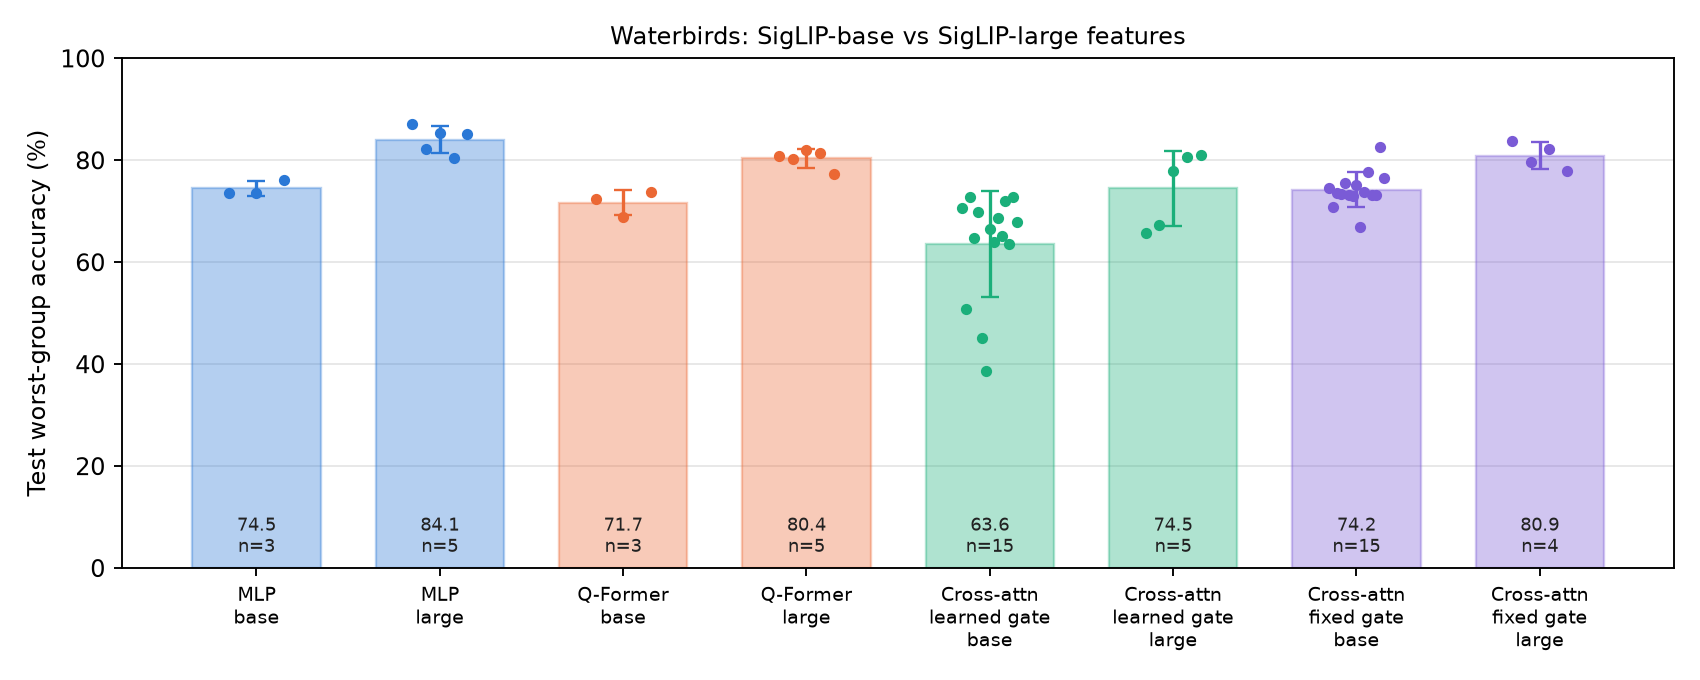
\includegraphics[width=\linewidth]{figures/encoder_scale.png}
\caption{Waterbirds worst-group accuracy with SigLIP-base and SigLIP-large features. Every connector gains from the larger encoder; the learnable gate still lags.}\label{fig:encoder}
\end{figure}

\begin{figure}[t]
\centering
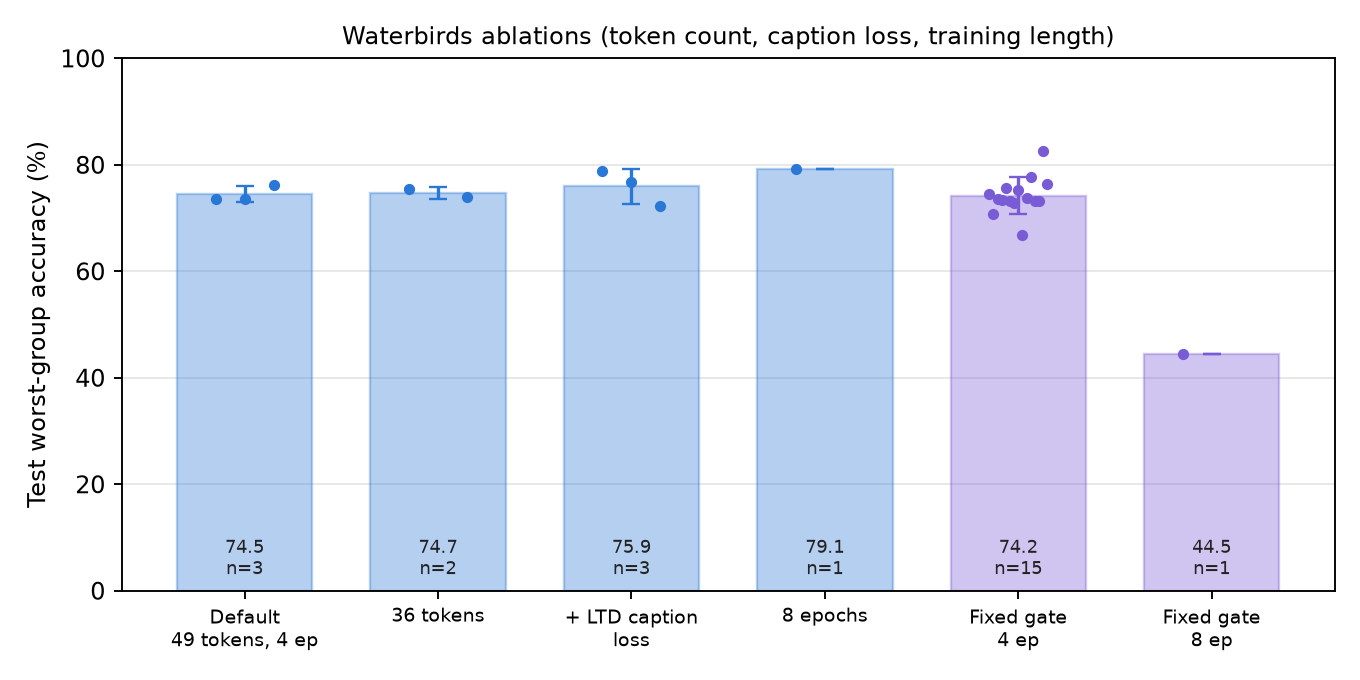
\includegraphics[width=0.85\linewidth]{figures/ablations.png}
\caption{Ablations on Waterbirds (MLP unless noted): image-token count, caption loss, training length, and the frozen-LLM control.}\label{fig:ablations}
\end{figure}

\subsubsection{Connector-only fixes}

Table 2, Figure 2: \texttt{docs/figures/final/fixes.png}. Stage-2 baseline vs connector-DFR, 5 seeds each:

{\def\LTcaptype{none} % do not increment counter
\begin{longtable}[]{@{}
  >{\raggedright\arraybackslash}p{(\linewidth - 10\tabcolsep) * \real{0.1379}}
  >{\centering\arraybackslash}p{(\linewidth - 10\tabcolsep) * \real{0.1724}}
  >{\centering\arraybackslash}p{(\linewidth - 10\tabcolsep) * \real{0.1724}}
  >{\centering\arraybackslash}p{(\linewidth - 10\tabcolsep) * \real{0.1724}}
  >{\centering\arraybackslash}p{(\linewidth - 10\tabcolsep) * \real{0.1724}}
  >{\centering\arraybackslash}p{(\linewidth - 10\tabcolsep) * \real{0.1724}}@{}}
\toprule\noalign{}
\begin{minipage}[b]{\linewidth}\raggedright
Task
\end{minipage} & \begin{minipage}[b]{\linewidth}\centering
Fixed gate
\end{minipage} & \begin{minipage}[b]{\linewidth}\centering
Fixed + DFR
\end{minipage} & \begin{minipage}[b]{\linewidth}\centering
MLP
\end{minipage} & \begin{minipage}[b]{\linewidth}\centering
MLP + DFR
\end{minipage} & \begin{minipage}[b]{\linewidth}\centering
Linear DFR (no LLM)
\end{minipage} \\
\midrule\noalign{}
\endhead
\bottomrule\noalign{}
\endlastfoot
Watermark & 72.5 ± 9.5 & \textbf{89.6 ± 0.5} & 64.9 ± 8.9 & 81.2 ± 2.2 & 85.1 ± 1.3 \\
Waterbirds & 73.9 ± 2.5 & 74.1 ± 5.6 & 74.9 ± 1.4 & 75.0 ± 3.6 & 84.2 ± 1.5 \\
\end{longtable}
}

\textbf{Watermark.}

\begin{itemize}
\tightlist
\item
  Connector-DFR raises fixed-gate WGA by 17.1 points.
\item
  It also reduces seed s.d. from 9.5 to 0.5.
\item
  Fixed + DFR exceeds MLP + DFR by 8.4 points (bootstrap 95\% CI {[}6.0, 9.8{]}; Holm-corrected hierarchical
  p \textless{} 0.001).
\end{itemize}

\textbf{Waterbirds.} Connector-DFR gives no gain, and every VLM stays about 10 points below linear DFR on the same
features.

\textbf{Other fixes.}

\begin{itemize}
\item
  Group-balanced sampling, which uses group labels in training, reaches 89.1 ± 0.9 (MLP) and 87.1 ± 3.5
  (fixed gate) on Watermark.
\item
  Connector-JTT (1 seed) did not help.
\end{itemize}

Figure \ref{fig:fixes} compares the connector-only fixes with group-balanced sampling and a linear probe on the same features.

\textbackslash begin\{figure\}{[}t{]}
\centering
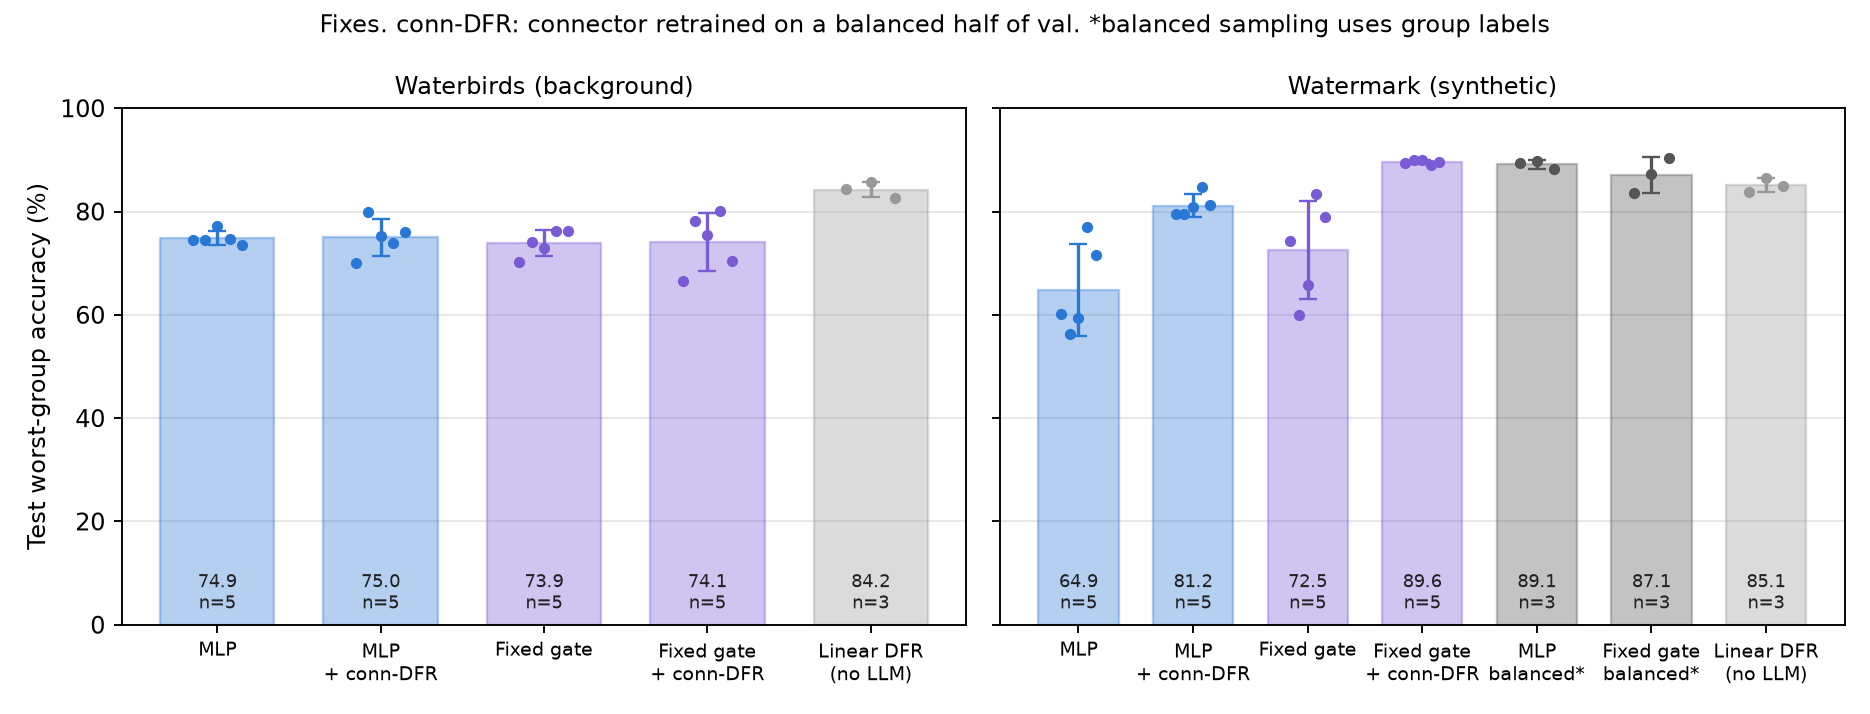
\includegraphics[width=\linewidth]{figures/fixes.png}
\textbackslash caption\{Connector-only deep feature reweighting (conn-DFR), group-balanced sampling and a linear DFR probe on the frozen features. Conn-DFR on the fixed gate reaches 89.6\% worst-group accuracy on the watermark task but gives no gain on Waterbirds.\}\label{fig:fixes}
\textbackslash end\{figure\}

\subsubsection{Generalisation to CelebA and to native VLMs (exploratory)}

\begin{itemize}
\item
  \textbf{CelebA} (8k-image stratified training subsample, so not comparable to full-data results): the ordering
  matches the other tasks, but no difference is significant:

  \begin{itemize}
  \tightlist
  \item
    MLP 54.3 ± 13.7 (4 seeds);
  \item
    learned gate 36.3 ± 18.7 (4 seeds);
  \item
    fixed gate 53.1 ± 5.8 (4 seeds); fixed − learned on 3 paired seeds +13.3, p = 0.24.
  \end{itemize}
\item
  \textbf{Native zero-shot:} Qwen3.5-4B with its own vision tower reaches 0.0 WGA (it always predicts one class),
  and 35.5 after a validation-calibrated threshold.
\end{itemize}

\subsection{Discussion}

\subsubsection{Overview}

A learnable injection gate, not the connector family, determines how strongly a generative VLM relies on a
shortcut:

\begin{itemize}
\tightlist
\item
  Fixing the gate open raised worst-group accuracy by 10--24 points with large effect sizes (\(d_z\) = 1.1--1.3).
\item
  It removed every collapsed seed.
\item
  The direction replicated on a second LLM.
\item
  Once the gate was fixed, MLP, Q-Former and cross-attention connectors were not significantly different.
\end{itemize}

\subsubsection{The gate as a transmission bottleneck}

\textbf{Finding.} The learned gate, initialised at zero, never opens during alignment, and models built on it rely
on the shortcut and vary widely across seeds.

\textbf{Comparison with the literature.}

\begin{itemize}
\item
  \emph{Gate closure:} this confirms \cite{farazi2026gate}, who found that learnable gates in frozen VLMs end up closed
  across five designs. We extend that observation from \emph{whether} the gate stays closed to \emph{what the model then
  relies on}, which they did not measure.
\item
  \emph{Feature--readout view:} the result also refines the decomposition of \cite{izmailov2022feature} and
  \cite{kirichenko2023dfr}. Between features and readout sits a transmission stage, and its failure produces
  shortcut reliance even when the features are adequate. Linear DFR on the same frozen features reaches about
  85 WGA.
\item
  \emph{Conflicting cross-attention evidence:} it helps explain why reports on cross-attention connectors disagree
  {[}laurencon2024matters vs farazi2026gate{]}. Averages over a few seeds hide a seed lottery: some learned-gate
  runs match the fixed gate, others collapse.
\end{itemize}

\textbf{Mechanism.}

\begin{itemize}
\item
  With \texttt{tanh(α)\ ≈\ 0}, unless \texttt{out\_proj} grows enough to offset it, the visual pathway contributes little to
  the language stream, so the LoRA-adapted LLM must fit the training labels from whatever survives. The
  injection ratio confirms a 15--35× weaker visual signal (R3).
\item
  On shortcut-aligned training data, the cue with the largest, most linearly available signal wins. This
  matches the ``easiest rule'' account of \cite{geirhos2020shortcut}.
\item
  Whether a run escapes depends on a near-zero gate with a sign-flipping gradient. That is a fragile,
  seed-dependent event, which is exactly what H2 predicts.
\item
  The frozen-LLM result supports this. Without LoRA to compensate, the learned gate falls to 24.2 WGA while
  MLP and Q-Former stay near 74.
\end{itemize}

\textbf{Scope relative to Flamingo.} Flamingo's gates ``quickly grow'' from zero over 500k steps with one gated block
every 4th--7th LM layer \cite{alayrac2022flamingo}. Our connector injects once, at the input embeddings, after 300
alignment steps. The finding is therefore scoped to short alignment and input-level injection, the regime of
adapter-style fine-tuning on a budget. Ten times longer alignment (3,000 steps) does not move it toward
Flamingo's behaviour: the gate stays shut. The learned-gate alignment then diverged (caption loss 2.0 → 7.9)
and its models collapsed (WGA 11.4 and 4.1 vs 70.8 and 59.5), so this run shows the learned gate is fragile
under longer training, but it is not a clean test of the gate alone. Flamingo also uses warmup, a smaller
learning rate for longer schedules and far more data, which we do not replicate. The IDEFICS gate
readings (9 of 20 layers below 0.05 after full training) show that near-shut gates also survive long training.
Flamingo also reports that removing the gate costs 4.2 points and destabilises training. Our fixed gate is not
``no gate'': the output layer is zero-initialised, so the model still starts as the pretrained LLM, and no
instability was observed.

\textbf{Relation to modality imbalance.} A gate that stays shut is a concrete, architectural instance of the
greedy under-use of one modality \cite{wu2022greedy} and of modality competition, in which the winner depends on
initialisation \cite{huang2022modality}. That account predicts the seed lottery we observe (H2). Prior work fixes
imbalance by modulating gradients \cite{peng2022balanced,wei2025onthefly}. Here, fixing one component removes the
problem at no cost, and the consequence is measured as worst-group accuracy rather than average accuracy.

\textbf{If the gate is shut, how is the visual shortcut learned?} The watermark and the background are themselves
visual, so some image signal must reach the LLM. A gate of ≈ 0.0005 passes little unless the output layer grows
to offset it. Our account is that the narrow residual pathway carries the strongest, most linearly available cue
and loses the finer object evidence. The injection ratio supports the first half: the pathway is open (the
injected signal is several times the text-embedding norm, because \texttt{out\_proj} grows) but 15--35× weaker than
with a fixed gate. Group DRO (R5) supports the second: with group-balanced weighting of the loss, the same
narrow pathway reaches 72.5 and 69.2 WGA, so it carries enough object evidence; under ERM the model does not
use it. The pathway ablation (round 5) adds the behavioural test. If ablation sends the learned-gate model to chance, the pathway is narrow but open. If it changes
nothing, the pathway is behaviourally closed and the shortcut comes from elsewhere.

\textbf{Behavioural closure.} \cite{farazi2026gate} define a pathway as closed when ablating it at inference leaves
accuracy unchanged, even when the gate nominally passes 30--45\% of the signal. Our gate value is a parameter
reading; the round-5 runs add their behavioural test (\texttt{ablated\_mean\_over\_templates}) and the injected-signal
ratio, so both criteria can be reported.

\textbf{Where the bias sits.} SpurLens attributes most of the spurious bias of MLLMs to the vision encoder
\cite{hosseini2025spurlens}. Our design holds the encoder fixed and shared across arms, so the gate effect cannot
come from the encoder; the two findings are complementary: the encoder decides what spurious information is
available, the connector decides how much of the rest reaches the LLM.

\textbf{Why not just use a linear probe?} Linear DFR on the same frozen features reaches about 85 WGA, above every
VLM (≈ 74). The study does not propose a better classifier; it explains a failure of VLMs. The gap is itself
evidence for the transmission account: the information is in the features but is lost between features and
answer.

\subsubsection{Attention is not reliance}

\textbf{Finding.} Both gate variants attend to the watermark about 2.5× more when it is present, yet only one relies
on it.

\textbf{Comparison.}

\begin{itemize}
\item
  Attention-based diagnostics of spurious features \cite{chakraborty2024exmap,lapuschkin2019clever} therefore
  need care in VLMs. This aligns with \cite{jain2019attention}.
\item
  It also shows the condition under which \cite{wiegreffe2019attention} expect attention to be informative:
  attention indicates reliance only when the pathway carrying it is open.
\end{itemize}

\textbf{Mechanism.} The learned gate multiplies attended features by \textasciitilde0.0005. Attention can be focused on the
watermark while transmitting almost nothing, so the shortcut reaches the answer through the LLM's own priors
and LoRA instead.

\subsubsection{Connector type is a weak factor for robustness}

\textbf{Finding.} With the gate pitfall avoided, MLP and Q-Former differ by under 3 points, and no comparison is
significant.

\textbf{Comparison.}

\begin{itemize}
\item
  This agrees with \cite{mckinzie2024mm1}, who found connector type matters little for benchmark accuracy, and
  with \cite{sarridis2026scaling}, who found data rather than architecture drives bias.
\item
  It is less consistent with \cite{huang2024mir}, whose MLP-over-Q-Former advantage in alignment quality does not
  appear as a robustness advantage here.
\end{itemize}

\textbf{Caveat.} Our TOST does not establish equivalence with 5 seeds, so the defensible claim is
\emph{no detectable difference}, not \emph{no difference}.

\subsubsection{A stronger encoder narrows the gap on Waterbirds but not on Watermark}

\textbf{Finding.} With SigLIP-large all connectors improve on Waterbirds, and the gate effect shrinks (74.5 vs 80.9,
paired +8.0, p = 0.09, 4 seeds), although the gate value is still 0.0006. On Watermark, 5 seeds give 53.2 vs 75.6
(+22.4, \(d_z\) = 0.85, p = 0.13, underpowered); the first two seeds alone had shown no gap (68.8 vs 68.2).
A shut gate is therefore not sufficient for shortcut reliance: it is a risk factor whose effect depends on the task
and on how separable the features are.

\textbf{Comparison.}

\begin{itemize}
\item
  This fits the encoder-centric account of MLLM failures \cite{tong2024eyes,tong2024cambrian}: better features
  help.
\item
  It also warns, in line with \cite{sagawa2020overparam}, that more capacity does not fix the mechanism.
\end{itemize}

\textbf{Mechanism.} Larger, more separable features let even a nearly closed pathway carry enough signal, or let
LoRA compensate. The fragility remains: one of five SigLIP-large learned-gate seeds still drops to 65.8 on Waterbirds.
Watermark seeds 2--4 (round 7) show the effect is still there.

\subsubsection{Readout fixes transfer to the connector, task-dependently}

\textbf{Finding.} Connector-DFR is the best label-light fix on Watermark (89.6, s.d. 0.5) but does nothing on
Waterbirds.

\textbf{Comparison.}

\begin{itemize}
\item
  This extends DFR \cite{kirichenko2023dfr} and its contrastive-VLM analogue \cite{you2024calibrating} to the connector
  of generative VLMs.
\item
  It also qualifies their premise that readout retraining suffices. It suffices when the shortcut is a
  localised, separable cue (a corner watermark). It does not suffice when the core and spurious features are
  entangled across the image (bird and background).
\item
  Linear DFR's Waterbirds advantage (84.2) shows the core information is present but not recoverable through
  this LLM readout with a few hundred balanced examples.
\end{itemize}

\subsubsection{Theoretical implications}

\begin{enumerate}
\def\labelenumi{\arabic{enumi}.}
\item
  \textbf{A transmission stage in the feature--readout account.} Shortcut reliance in modular models can arise
  between features and readout, through what an interface lets through. The gate is a concrete, measurable
  instance.
\item
  \textbf{Variance as an outcome.} Architectural choices can change \emph{how often} a model learns the shortcut, not
  only how much on average. Seed-level reporting is therefore required for claims about robustness
  \cite{bouthillier2021variance}.
\item
  \textbf{A cost of near-identity initialisation.} Zero- or small-initialised learnable residual scales are
  standard because they stabilise optimisation \cite{bachlechner2021rezero,de2020skipinit,touvron2021cait}.
  That literature measures convergence and average accuracy in unimodal networks, where each scaled branch
  sees the same input. When the scaled branch is the only path for a modality, the same initialisation has a
  robustness cost: the branch stays small and the model relies on the shortcut. The design question is
  therefore not only how to start near the identity, but through which parameter (gate vs output layer).
\item
  \textbf{A boundary condition for readout fixes.} Connector-level DFR works when the spurious cue is spatially
  localised and separable, and fails when it is entangled with the core object.
\end{enumerate}

\subsubsection{Practical implications}

\begin{itemize}
\item
  \textbf{Fixed injection:} prefer fixed (or zero-initialised-output) injection over learnable tanh gates when
  adding cross-attention adapters to an LLM. Log the gate value if a learnable gate is kept.
\item
  \textbf{Where it sits among fixes:} label-using methods (Group DRO, group-balanced sampling, connector-DFR) reach
  similar or higher WGA. The fixed gate's advantage is that it needs no group labels, no extra training and no
  extra compute, so it should be the default, with label-using fixes added when labels exist. It removes
  one cause of failure, not all: on Phi-4-mini Watermark 6 of 10 fixed-gate seeds still fall below 50\%.
\item
  \textbf{Evaluation:} evaluate worst-group accuracy over at least 5--10 seeds before choosing a connector.
\item
  \textbf{Cheap fix:} when a small group-balanced set exists, retrain only the connector. It costs one epoch, needs
  no LLM retraining, and stabilises seeds.
\item
  \textbf{Cost:} the fixed-gate cross-attention connector matches MLP robustness at about half the step time and
  memory (1.7 vs 4.0 s per step; 6.2 vs 12.1 GB on a T4).
\end{itemize}

\subsubsection{Open-ended answers on natural images (VQA-CP v2): the gate effect does not appear}

\textbf{Finding.} On a VQA-CP v2 subset (8k training questions, 3 epochs, 3 seeds) the fixed gate is worse than the
learned gate: test-ID VQA accuracy 42.6 vs 47.6 (p = 0.010) and shifted-prior accuracy 27.6 vs 29.1 (p = 0.054,
paired, exploratory). Both arms lose 15--19 points when the priors shift (ID − OOD 18.5 and 15.0), so the benchmark does
expose the language prior.

\textbf{What the pathway test shows.} Removing the image changes nothing for the learned gate (47.6 → 47.6; 29.1 → 29.2),
so it is effectively a text-only model here, with injection ratio 0.05. It answers with the training prior more
often (39.9\% vs 33.8\% in distribution), which is the direction the mechanism predicts. The fixed gate uses the image
slightly (−2.2 points without it in distribution) but its injected signal is about 70× the text norm, and removing it
\emph{raises} shifted-prior accuracy by 4.6 points (27.6 → 32.2).

\textbf{Interpretation.} Of the three predictions (lower shifted-prior accuracy for the learned gate, more prior answers,
smaller loss without the image), only the last two hold. At this training scale neither connector learns to use the
image beyond the language prior, and a strong injection disturbs free-form answer generation. We therefore do not
claim that the gate effect transfers to open-ended VQA. There is no connector-free text-only baseline, so the
amount of image information used cannot be bounded from this run.

\subsubsection{Limitations and future research}

\textbf{Limitations.}

\begin{itemize}
\item
  Models are 4-bit and 4B parameters or smaller.
\item
  The encoder is frozen.
\item
  SigLIP-large Watermark has 5 seeds, CelebA 5 paired, the 8-epoch runs 4--5, the pathway ablation 1--2 seeds.
\item
  The three classification tasks are binary questions answered by the first token of the class word. Open-ended
  generation is tested only on a VQA-CP v2 subset (3 seeds), not on the full benchmark, and there the gate
  effect did not appear (D10).
\item
  Runs are not bit-reproducible: same-seed reruns differ by 12.7 (learned) and 5.2 (fixed) WGA points on
  average, so seeds are treated as random replicates.
\item
  The learning-rate sweep has 2 seeds per setting (the third seed did not run) and is descriptive; Group DRO has 4.
\item
  The open-gate control separates initialisation from learnability only partly: at α = 3 the gate gradient
  is scaled by 1 − tanh² ≈ 0.01, so the open gate barely moves.
\item
  One of five fixed-gate 8-epoch runs collapsed (44.5), so long training can hurt the fixed gate occasionally.
\item
  CelebA trains on an 8k subsample.
\item
  Group DRO is the only full-model group-robust baseline; JTT is tested only at the connector.
\item
  Phi-4-mini Watermark is underpowered (0.40).
\item
  The Watermark shortcut is partly textual \cite{materzynska2022disentangling}.
\item
  Equivalence of connector types is not established.
\item
  Injection is input-level (one block), not per-layer as in Flamingo, and alignment is 300 steps.
\item
  In stage 2 the learned gate has weight decay 0.01 (none in alignment); it shrinks α by a relative
  2 × 10⁻⁶ per step (lr × decay), negligible, and a no-weight-decay control is in round 5.
\item
  Watermark uses one shortcut strength (p = 0.95); a dose--response at p = 0.9 and 0.99 is in round 5.
\item
  SigLIP's web pre-training may include CUB, Places or COCO images (shared by every arm).
\item
  CelebA and Waterbirds are licensed for non-commercial research only.
\end{itemize}

\textbf{Three directions for future work.}

\begin{enumerate}
\def\labelenumi{\arabic{enumi}.}
\item
  Test gate dynamics in full-precision, larger models with trainable encoders: IDEFICS-scale models and
  Llama 3 vision adapters \cite{grattafiori2024llama3}.
\item
  Design injection schemes that start as the identity but cannot close, and test them on natural-image
  benchmarks of spurious cues \cite{yang2025spuriverse,hosseini2025spurlens}.
\item
  Explain why connector-DFR fails on entangled shortcuts, for example with subspace explanations
  \cite{chormai2024disentangled}, and combine it with data-level fixes \cite{noohdani2024decompose}.
\end{enumerate}
